\documentclass[12pt,fleqn]{article}\usepackage{../common}
\begin{document}

\begin{minted}[fontsize=\footnotesize]{python}
G1 = {
  'a': {'b':1, 'f':2, 'g': 6},
  'b': {'a':1, 'c':1},
  'c': {'b':1},
  'd': {'f':1, 'e':2},
  'e': {'d':2, 'g':1},
  'f': {'a':2, 'd':1},
  'g': {'e':1, 'a': 6}
}
\end{minted}

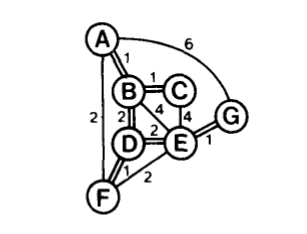
\includegraphics[height=4cm]{minspan_0.png}

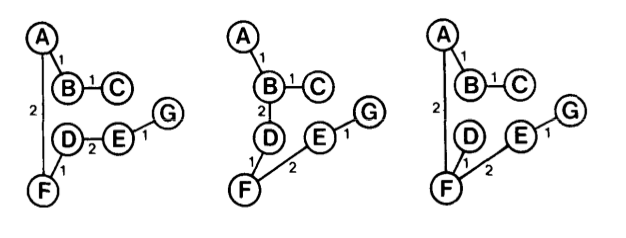
\includegraphics[height=4cm]{minspan_1.png}


\begin{minted}[fontsize=\footnotesize]{python}
def find(C, u):
    if C[u] != u:
        C[u] = find(C, C[u])                    # Path compression
    return C[u]

def union(C, R, u, v):
    u, v = find(C, u), find(C, v)
    if R[u] > R[v]:                             # Union by rank
        C[v] = u
    else:
        C[u] = v
    if R[u] == R[v]:                            # A tie: Move v up a level
        R[v] += 1

def kruskal(G):
    E = [(G[u][v],u,v) for u in G for v in G[u]]
    T = set()
    C, R = {u:u for u in G}, {u:0 for u in G}   # Comp. reps and ranks
    print sorted(E)
    for _, u, v in sorted(E):
        if find(C, u) != find(C, v):
            T.add((u, v))
            print (u, v)
            union(C, R, u, v)
    return T

print list(kruskal(G1))
\end{minted}

\begin{verbatim}
[(1, 'a', 'b'), (1, 'b', 'a'), (1, 'b', 'c'), (1, 'c', 'b'), (1, 'd', 'f'), (1, 'e', 'g'), (1, 'f', 'd'), (1, 'g', 'e'), (2, 'a', 'f'), (2, 'd', 'e'), (2, 'e', 'd'), (2, 'f', 'a'), (6, 'a', 'g'), (6, 'g', 'a')]
('a', 'b')
('b', 'c')
('d', 'f')
('e', 'g')
('a', 'f')
('d', 'e')
[('d', 'e'), ('e', 'g'), ('d', 'f'), ('b', 'c'), ('a', 'f'), ('a', 'b')]
\end{verbatim}

\begin{minted}[fontsize=\footnotesize]{python}
m = 100 * 1000
print m**2
print np.log(m)
print m*np.log(m)
\end{minted}

\begin{verbatim}
10000000000
11.512925465
1151292.5465
\end{verbatim}


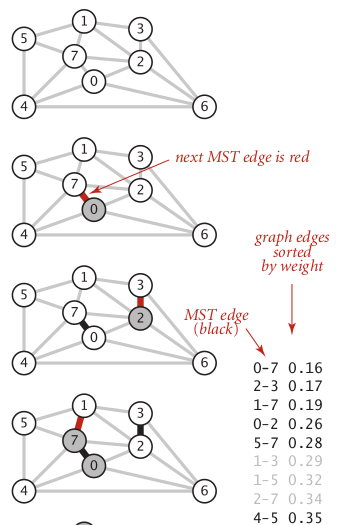
\includegraphics[height=9cm]{sedge_krus_1.png}

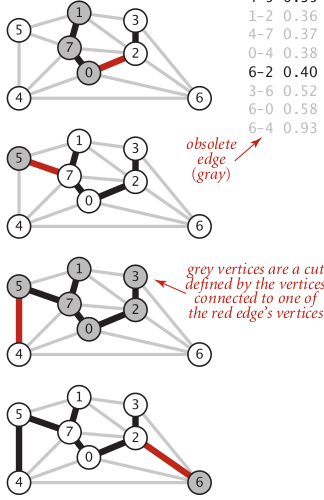
\includegraphics[height=9cm]{sedge_krus_2.png}


\begin{minted}[fontsize=\footnotesize]{python}
G2 = {
  0: {7: 0.16, 4: 0.38, 2: 0.26, 6: 0.58},
  1: {5: 0.32, 2: 0.36, 3: 0.29, 7: 0.19},
  2: {0: 0.26, 1: 0.36, 3: 0.17, 6: 0.40, 7: 0.34},
  3: {1: 0.29, 2: 0.17, 6: 0.52},
  4: {0: 0.38, 5: 0.35, 7: 0.37, 6: 0.93},
  5: {1: 0.32, 4: 0.35, 7: 0.28},
  6: {0: 0.58, 2: 0.40, 3: 0.52, 4: 0.93},
  7: {0: 0.16, 1: 0.19, 5: 0.28, 4: 0.37, 2: 0.34, 1: 0.19}
} 

print list(kruskal(G2))
\end{minted}

\begin{verbatim}
[(0.16, 0, 7), (0.16, 7, 0), (0.17, 2, 3), (0.17, 3, 2), (0.19, 1, 7), (0.19, 7, 1), (0.26, 0, 2), (0.26, 2, 0), (0.28, 5, 7), (0.28, 7, 5), (0.29, 1, 3), (0.29, 3, 1), (0.32, 1, 5), (0.32, 5, 1), (0.34, 2, 7), (0.34, 7, 2), (0.35, 4, 5), (0.35, 5, 4), (0.36, 1, 2), (0.36, 2, 1), (0.37, 4, 7), (0.37, 7, 4), (0.38, 0, 4), (0.38, 4, 0), (0.4, 2, 6), (0.4, 6, 2), (0.52, 3, 6), (0.52, 6, 3), (0.58, 0, 6), (0.58, 6, 0), (0.93, 4, 6), (0.93, 6, 4)]
(0, 7)
(2, 3)
(1, 7)
(0, 2)
(5, 7)
(4, 5)
(2, 6)
[(2, 6), (4, 5), (5, 7), (0, 7), (2, 3), (1, 7), (0, 2)]
\end{verbatim}


















Sedgewick, R. {\em Algorithms}, sf. 409

Sedgewick, R. {\em Algorithms, 4rd Edition}, sf. 624

Heatland, Python Algorithms

\end{document}
